%! Author = sbbfti
%! Date = 10/06/2020

\section{Methodology}\label{sec:methodology}

The energy balance model estimates how environmental (i.e., \ac{t-db}, \ac{t-r}, \ac{v}, \ac{rh}) and personal factors (i.e., \ac{clo}, \ac{met}) influence both latent and sensible components of the \ac{q-sk}, and the \ac{q-res}.
Moreover, it can be used to estimate the value of some physiological variables such as \ac{t-sk}, and \ac{t-cr}.
% note OJ Our perspective on this is that for determining environmental limits a fixed maximum Tsk value (associated with complete vasodilation) is sufficient, and less complicated
\ac{v} is the average air speed of the flow that is used to cool the human body~\cite{Huang2014}.
% note OJ Similarly, the absolute Tcore was previously not considered important to determine, rather whether the condition was uncompensable or not was thought to be most important as this does not require us to estimate exposure time

Section~\ref{subsec:energy-balance} describes the main Equations used by the model to derive the results.

\subsection{Energy Balance}\label{subsec:energy-balance}

The human body exchanges both sensible and latent heat with its surrounding environment.
Sensible heat is transferred via conduction, convection and radiation (\acs{c-r} + \acs{c-res}).
While latent heat loss occurs from the evaporation of sweat (\acs{e-rsw}), moisture diffused through the skin  (\acs{e-dif}), and respiration (\acs{e-res})
The energy balance in the human body is described by:

\begin{equation}
    M - W = C + R + E_{sk} + C_{res} + E_{res} + S_{sk} + S_{cr}\label{eq:heat-balance}
\end{equation}

This equation assumes that the body comprises two main thermal compartments: the skin and the core.
If the exogenous and endogenous heat gains cannot be compensated by heat loss, then both the \ac{s-sk}, and the \ac{s-cr} increase and in turn the \ac{t-sk}, and \ac{t-cr} rise, respectively.
One of the main differences between our proposed model and the one used by \mycite{Jay2015} is that their model does not account for heat stored in the core or the skin compartment, hence, they assume the values of \ac{t-sk} and \ac{t-cr} to be constant.
% note OJ - See previous comment. Tcr was not necessarily fixed, rather the heat balance equation was solved for when Ereq exceeded Emax (with certain physiological limits), i.e. when uncompensable.
Calculating how \ac{t-sk} and \ac{t-cr} vary as a function of different environmental and personal factors allows us to better predict how much heat the body exchanges with its surrounding environment.
% note OJ - I would say that this is not necessarily correct. Tsk will modify dry heat loss (a little bit) but at the point of compensability tsk will be max, so a simplified model can just assume max Tsk with full vasodilation (35.5˚C). Absolute Tcore does not really drive sweat rate, Ereq does: see Ravanelli & Jay (2020) J Physiol (London).

The amount of sensible heat gains or losses from the human body to its environment can be expressed as a function of environmental (\ac{t-db}, \ac{t-r}, \ac{v}, and \ac{rh}), and personal factors (\ac{met}, and \ac{clo})~\cite{ASHRA2017}.
% note OJ - Based on this text it is not clear how Tcr modifies heat exchange as stated n the previous paragraph - I don't think it should.

The equations used to determine sensible and latent heat loss are based on fundamental heat transfer theory, while the coefficients were estimated empirically~\cite{ASHRA2017}.

\subsubsection{Body Surface Area}

All the terms presented in Equation~\ref{eq:heat-balance} are reported in power per unit of human \ac{body-a}.
Equation~\ref{eq:dubois} can be used to estimate \ac{body-a} as a function of the \ac{body-w} and \ac{body-h}~\cite{DuBois}.

\begin{equation}
    A_{body} = 0.202 mass^{0.425} height^{0.725}\label{eq:dubois}
\end{equation}

In thermal comfort research, this value is generally assumed to be constant and equal to 1.8 m$^{2}$.
\mycite{Jay2015} also consider this value to be constant, however, it should be noted that this is an approximation.
Several other equations have been developed to estimate \ac{body-a} and in the function of the \verb|pythermalcomfort| tool, we allow users to specify \ac{body-a} as the input value.
Alternative equations to the DuBois equation are available.
A review paper concluded that most of the proposed equations in the literature were in agreement with each other to estimate \ac{body-a} for adults with a healthy weight and standard physique~\cite{Redlarski2016}.

\subsubsection{Sensible Heat Loss from Skin}

Sensible heat loss from the human body mainly occurs from convection and radiation from the skin to the environment.
The total amount of \ac{c-r} can be described as a function of \ac{t-sk}, \ac{t-op}, \ac{r-cl}, \ac{f-cl}, and \ac{h}.
The equation can be expressed as:

\begin{equation}
    C+R=\frac{t_{s k}-t_{o}}{R_{c l}+1 /\left(f_{c l} h\right)}\label{eq:c-r}
\end{equation}

\begin{equation}
    f_{cl}=1.0 + 0.31 I_{cl} \label{eq:f-cl}
\end{equation}

\begin{equation}
    h=h_{c} + h_{r} = \max(3, 8.6 V^{0.53}) p_{atm}^{0.53} + 4 \varepsilon \sigma \frac{A_{\mathrm{r}}}{A_{body}}\left[273.2+\frac{\left(t_{\mathrm{cl}}+\overline{t_{r}}\right)}{2}\right]^{3}\label{eq:h}
\end{equation}

Where the ratio between \ac{a-r} and \ac{body-a} is assumed to be 0.70 for a sitting person and 0.73 for a standing person~\cite{Fanger1967}.
The \ac{e} is close to unity (typically 0.95) and the \ac{sigma} is a constant.
The value of \ac{t-op} varies as a function of the \ac{h-c}, \ac{h-r}, \ac{t-r} and \ac{t-db}, and it is described by:

\begin{equation}
    t_{o}=\frac{h_{r} \bar{t}_{r}+h_{c} t_{db}}{h_{r}+h_{c}}\label{eq:t-op}
\end{equation}

In our model, the value of \ac{t-sk} is calculated iteratively since it varies as a function of the heat loss from the human body towards its environment and the heat transferred from the core to the skin node, as shown in Source Code~\ref{lst:pythonCode}.
\Ac{t-cl} can be calculated as a function of \ac{t-op}, \ac{t-sk}, \ac{r-cl} and the resistance of the air layer.
% note OJ - Is the disruption of the air layer with fanning and subsequent alteration in insulative/evaporative resistance properties accounted for

\subsubsection{Latent Heat Loss from Skin, (\acs{e-sk})}

The \acf{e-sk} comprises two terms: the \ac{e-rsw} and the \ac{e-dif}.
\ac{e-sk} depends on the \ac{w}, \ac{p-sk} normally assumed to be that of saturated water vapor at \ac{t-sk}, \ac{p-a}, \ac{f-cl}, \ac{h-e}, and \ac{r-e-cl}.

\begin{equation}
    E_{s k}=E_{rsw}+E_{dif}=\frac{w\left(p_{s k, s}-p_{a}\right)}{R_{e, c l}+1 /\left(f_{c l} h_{e}\right)}\label{eq:latent-skin}
\end{equation}

Despite the fact that Equation~\ref{eq:latent-skin} is expressed as a function of \ac{w}, the human body does not regulate \ac{w} directly but, rather, it regulates the sweat rate.
% note OJ - I know this might sound crazy, but I am not sure this is correct - which might be a problem with model. Physiological evidence points to the evaporative heat loss requirement for heat balance being the regulated variable - in a sense, i.e. this is what determines the steady-state SR. The onset and thermosensitivity of the thermoeffector response determines how hot someone gets before they reach steady-state.
%We recently published a paper on this in J Physiol (London):
%Ravanelli N, Imbeault P, Jay O (2020) Steady-state sweating during exercise is determined by the evaporative requirement for heat balance independently of absolute core and skin temperature. J Physiol (London); 598(13):2607-2619.
%With an editorial: Mundel T (2020) Thermoregulatory sweating and evaporative heat loss during exercise: is the whole greater than the sum of its parts? J Physiol (London); 598(13):2535-2536.
%This is further modified by skin temperature. See our recent paper in MSSE:
%Hospers L, Cheuvront S, Kenefick RW, Jay O* (2020) Independent influence of skin temperature on whole-body sweat rate. Med Sci Sports Exerc; 52(11):2423-2429.
%
%...which is why I think you can get lower core temperature with a higher sweat rate with fan use in some conditions (e.g. the 40C/50%RH condition of Morris et al 2019).

Skin wettedness varies as a function of the activity of the sweat glands and the environmental conditions.
It correlates with warm discomfort and is a good measure of thermal stress.
While \ac{w} can theoretically range from 0 to 1 and skin wettedness can approach 1.0 while the body still maintains thermoregulatory control~\cite{ASHRA2017}.
In most situations, the upper limit of \ac{w} is lower than 1.
\mycite{GaggeSET} used the following equations to determine \ac{w-max} for sustained activity for healthy and acclimatized humans:

% todo ED There are physiological sweat rate control equations that affect wmax, right? Do they need to be described?

\begin{equation}
    w_{max}=
\begin{cases}
    0.38 V^{-0.29} & \text{if } I_{cl} = 0 \text{ (i.e., naked)} \\
    0.59 V^{-0.08} & \text{if } I_{cl} > 0
\end{cases}
\end{equation}

On the other hand, \mycite{Jay2015} adjusted the value of \ac{w-max} based on fan use and age.
For young adults, they assumed \ac{w-max} to be equal to 0.65 for the `fan on' condition and 0.85 for the `fan off' condition.
% todo add references
These values are higher than those estimated by the \mycite{GaggeSET} model.
% note OJ I might be missing it but I am not clear where how sweating efficiency has been accommodated? As discussed on our call, at lower RH values sweat efficiency approaches 100% even with a fan so fan just add dry heat (if Ta>Tsk) without much increase in evaporation -this causes the real Ta/RH threshold curve for fan use to bend downwards to lower temperature (on the y-axis) at lower humidity values. I think this would be very important to include.

\subsubsection{Respiratory Losses, (\acs{q-res})}
The human body exchanges both sensible and latent heat with its environment.
The \acf{q-res} equals the sum of the \ac{c-res} and the \ac{e-res}.
The value of \ac{q-res} is can be determined using the following simplified equation~\cite{ASHRA2017}:

\begin{equation}
    q_{res} = C_{res} + E_{res} = 0.0014M(34-t_{a}) + 0.0173M(5.87-p_{a})\label{eq:respiratory-losses}
\end{equation}

\subsection{Data Analysis}\label{subsec:data-analysis}

The heat balance model was used to estimate sensible and latent heat loss and several physiological parameters (e.g., \ac{m-sweat}, \ac{t-cr}).
We calculated the results for \ac{t-op} ranging from 28 to 55~$^{\circ}$C at 0.5~$^{\circ}$C intervals, \ac{rh} ranging from 0 to 100~\% at 5~\% intervals and for the discrete values of \ac{v} = 0.2, 0.8 and 4.5~m/s.
In this paper, we will be referring to `still air' condition when air velocities are below \ac{v}~=~0.2 m/s.
This definition is in accordance with the ASHRAE 55--2017 Standard~\cite{ashrae552017} and allowed us to compare our results with those obtained by \mycite{Jay2015}.
We assumed \ac{t-r} to be equal to \ac{t-db}, \ac{clo}~=~0.5~clo, and \ac{met}~=~1.1~met, unless otherwise specified.
It could be argued that some people during heatwaves may be wearing fewer clothes than that, hence, a value of \ac{clo} equal to 0.36 clo (i.e., walking shorts, short-sleeve shirt, and sandals) would be more appropriate, however, we wanted to use a more conservative value.
Results for different combinations of environmental and personal conditions can be generated using our online tool.
In this manuscript, we assumed the \ac{i-cl} to be constant and equal to 1 and 0.45, as assumed by \mycite{GaggeSET}, for naked and clothed people, respectively.
Users can, however, change this value in the source code.
We report heat losses per unit of skin surface area.
Thermal strain is assumed to occur when either of the following parameters reach their maximum value: \ac{w}, skin blood flow, or \ac{m-sweat}.
The former assumption is based on the fact that there is a \ac{w-max} for sustained activity for healthy and acclimatized humans~\cite{ASHRA2017}.
The other two assumptions are based on the fact that \mycite{GaggeSET} state that serious danger of fatality exists when blood flow from the core to the skin is maximal or sweating reaches its maximum.
We assumed that the use of electric fans is detrimental when the value of \ac{t-cr} calculated for values of \ac{v} higher than 0.2~m/s exceeds the value determined for the `still air' condition.

Results were calculated using the  \verb|pythermalcomfort| Python package~\cite{Tartarini2020a} function \verb|use_fans_heatwaves|.
A copy of the algorithm we used to calculate the results can also be found in \ref{sec:python_code}.
Lines in Figures~\ref{fig:comparison_models}, \ref{fig:results_model_2}, \ref{fig:comparison_air_speed}, \ref{fig:met_clo}, \ref{fig:energy_storage_delta}, and \ref{fig:use_fans_and_population} were smoothed using the \verb|Scipy| function \verb|ndimage.gaussian_filter1d|.
Moreover, we developed a tool that can be used to generate interactive figures that show the environmental conditions under which the use of elevated air speeds is beneficial.
This tool has been added and integrated into the CBE Thermal Comfort Tool~\cite{Tartarini2020}.

\subsection{Weather Data}\label{subsec:weather-data}

To better understand in which locations worldwide the use of electric fans would be beneficial we compared the results obtained from the heat balance model with the climatic data provided in the 2017 ASHRAE Handbook--Fundamentals~\cite{ASHRA2017} and the records from the Emergency Events Database (EM-DAT) which contains a list of the deadliest heatwaves recorded from 1936 to the present date~\cite{EMDATThe70:online}.

From the ASHRAE climatic design dataset extracted weather data from more than 5000 stations worldwide.
For each station we collected the: maximum extreme \ac{t-db} with a 20 year return period;
and the \ac{t-db} corresponding to the hottest 0.4~\% of annual cumulative frequency of occurrence and the mean coincident \ac{t-wb}.
For more information about the ASHRAE climate design dataset please refer to Chapter 14 of the 2017 ASHRAE Handbook--Fundamentals~\cite{ASHRA2017}.
The location of the stations and their respective maximum extreme dry-bulb temperatures are shown in Figure~\ref{fig:world-map}.
We do not show data from stations with a maximum temperature lower than 26~$^\circ$C\@ since we are only interested in assessing the benefit of using fans during hot days.

\begin{figure}[thb!]
    \centering
    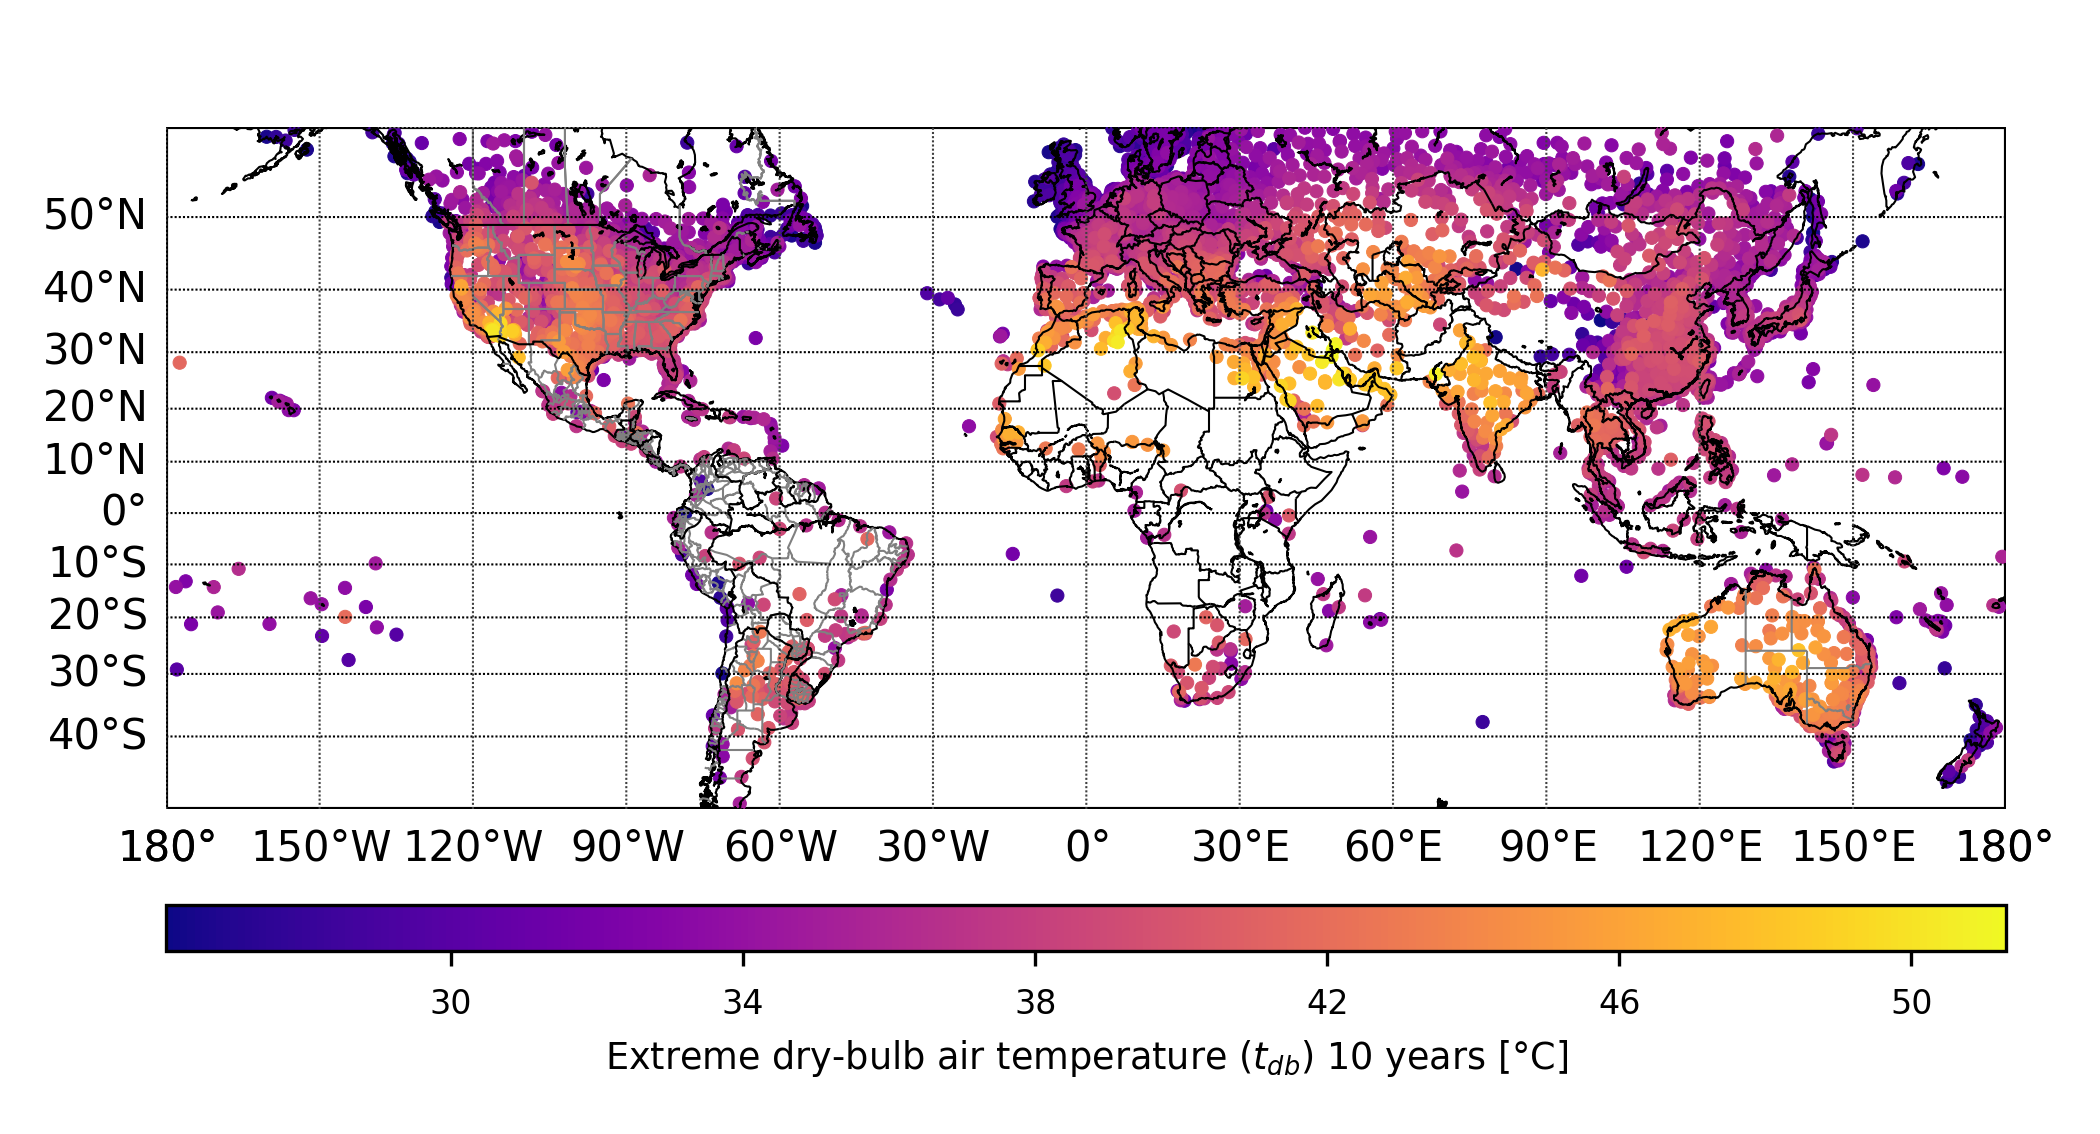
\includegraphics[width=\textwidth]{figures/world-map}
    \caption{Shows the location of each weather station that was included in the analysis and the maximum extreme dry-bulb temperature with a 20 year return period.}
    \label{fig:world-map}
\end{figure}

Few data are available for Sub-Saharan Africa where approximately 40~\% of the poorest people in the world reside and where climate change may be an acute threat~\cite{PovertyO1:online}.

In order to determine the coincident value of \ac{rh} when the maximum extreme \ac{t-db} with a 20 year return period was recorded we used the following two methods:

\textit{Constant humidity ratio} -- Firstly, we determined the humidity ratio for each location based on using the following temperatures the \ac{t-db} corresponding to the hottest 0.4~\% of annual cumulative frequency of occurrence and the mean coincident \ac{t-wb}.
We then assumed that during an heatwave the humidity ratio would remain constant while only the value of \ac{t-db} would increase.
This assumption allowed us to estimate, for each location, the value of \ac{rh} for each extreme \ac{t-db}.
This is an approximation and it does not take into account that during heat waves the value of humidity ratio could increase.

\textit{Coincident extreme conditions} -- In parallel we also estimated the value of \ac{rh} using the maximum extreme \ac{t-db} and \ac{t-wb} reported in the ASHRAE climate design dataset for each location.
This method assumes that both temperatures would occur at the same time in each location.
This is an approximation and it is arguably overestimating the most extreme condition because the likelihood of both conditions occurring at the same time is extremely low.

We compared the results, obtained using both models, to the data that \mycite{Hospers2020} reported in their manuscript.
\mycite{Hospers2020} obtained hourly data for the 100 most populous metropolitan areas in the U.S. from January 1st, 2000 to December 31st, 2019.
They purchased the data from fromCustomWeather (CustomWeather, Inc., 271Miller AvenueMill Valley, CA, USA 94941).
From this dataset they determined the peak \ac{t-db} and corresponding \ac{rh} for each location.
Results of this comparison are presented in \ref{sec:validation_rh}.
We concluded that the constant humidity ratio assumption led to more accurate results than the other proposed method.

We also assumed that during heatwaves \ac{t-db} and \ac{rh} indoors would be equal to \ac{t-db} and \ac{rh} outdoors.
Conditions indoors may, however, be slightly less severe than outdoors since the thermal mass of the building may dump and shift peaks in outdoor temperature.
% note OJ We just got pilloried for this same approach in our modeling paper for estimating the GHG reductions due to AC use by increasing the upper temperature for TC with increasing air speeds (submitted for ERL). We did not have this problem with our other recent submission to Lancet Planetary Health. In any case, it would be good include more detail supporting this rationale including some references.
At the same time, the opposite scenario can also occur if there is a significant amount of internal load or solar gains indoors.

The EM-DAT contains detailed information on when the heatwave occurred, the location, the number of deaths, and the maximum temperature recorded.
However, it does not contain information about the \ac{rh} which is important for determining whether the use of electric fans would have been beneficial or not.

\subsection{City Population Data}\label{subsec:population-data}

% note OJ Just FYI. We have taken a similar approach in our recent Lancet PH submission. We have 110 cities from 6 continents and specifically selected some of them based on the project AC use according to Davis et al (2015) PNAS.

We obtained the city population data from the demographic statistics database which is compiled and maintained by the \ac{un} statistics division~\cite{UNdatare88:online}.
The database was last updated in August 2020 and we used it to gather information about the number of people who live in the 115 most populous cities in the world.
When available we used the population of the urban agglomerate rather than of the city administrative boundary.
We then combined the population with the ASHRAE weather data to determine during extreme heat events: i) how many people were at high risk of experiencing \ac{t-db} higher than 35~$^{\circ}$C\@, and ii) how many people would benefit from the use of electric fans.
As mentioned in Section~\ref{subsec:weather-data} weather data were not available for all the major cities in the world.
Consequently, we had to exclude the following cities from our analysis: Lagos in Nigeria, Dar es-Salaam and Mwanza in Tanzania, Dhaka in Bangladesh, Faisalabad in Pakistan, Zibo and Zhongshan in China, Addis Ababa in Ethiopia, and Bandung in Indonesia.
A full list of the cities we included in the analysis is provided in the \ref{sec:pop_weather}.

\subsection{Elderly}\label{subsec:elderly}

% todo say something how we calculated w_crit for the elderly